% Author @ Sam Appleton, IN_PROGRESS, Reviewer @ Jeremy Perez, Due Date 11/11

This chapter discusses our implementation in determining the difficulty of 
the Maximum Matching problem. This includes a summary of created programs,
an explanation of implemented solvers, our development tools, and a 
discussion on parallel programming. 

\section{Implementation}
Understanding the difficulty of Maximum Matching requires exploration via 
implementation. Our implementation includes various solvers and tools for answering
the question of Maximum Matching. In this section, we summarize and describe
each part of the implementation. 

Our implementation includes:
\begin{itemize}
	\item \textbf{Benchmarking}: Tools that determine the running time of 
    each solver algorithm. They take in a series of tests and a solver, and then
    return the correctness of the results and the wall-clock time of each solved test.
	\item \textbf{Solvers}: Algorithms that find the maximum matching on a given
    graph instance. They include many different types of solvers which implement
    different programming styles, such as integer programming and heuristics. 
	\item \textbf{Test Generators}: Tools for creating graph instances. They 
    generate random graphs with known maximum matchings for the sake of testing 
    correctness and efficiency. 
	\item \textbf{Visualizer}: Tool for creating visual representations of
    graph instances. It provides access for humans to interpret the graph objects,
    which are hard to easily understand. 
\end{itemize}

\section{Benchmarking} \label{BenchmarkingSummary}
Benchmarking is crucial to our implementation. It allows us to determine the efficiency 
of our solvers, thus giving an empirical way of comparing solvers. 
Our benchmarking tool takes in a series of graphs and runs each of them against a solver that
finds the maximum matching on each graph.
It then determines the accuracy of the solver by comparing the returned maximum matching and 
seeing if it is valid. It also records the wall-clock time needed for each graph
in the input to compare the running times of each solver. Each graph is represented 
in a .mmi (Maximum Matching Instance) file, and the files paths to each graph 
is stored in a .mmb (Maximum Matching Benchmarking) file. This allows .mmb files to be created
with specific factors in mind, such as only containing dense graphs with $d > 2$. This program
is essential to our understanding of the hardness of Maximum Matching as it gives a 
quantifiable determinant of difficulty, that being the actual time it take to solve a given 
instance of the problem. Calculating running time on the same machine with the same environment
allows us to easily compare different implementations. 

A .mmi file contains a single graph object as represented by the following lines:
\begin{enumerate}
	\item $d$, an integer that represents the number of dimension in the graph. 
	\item $n$, an integer that represent the number of vertices in each dimension.
	\item $m$, an integer that represents the number of edges in the graph.
	\item $m$ tuples of length $d$ that contain numbers $(1..n)$ that represent
	each edge on the graph.
	\item $M$, an integer that represents the cardinality of the known maximum matching 
    of the graph. Note that this line is optional.
\end{enumerate}
Figure \ref{fig:exampleMMi} contains an example .mmi file, and Figure \ref{fig:d4v5} contains 
a visualization of the corresponding output.

\begin{figure}[t!]
    \centering
    \begin{minipage}{0.45\textwidth}
        \centering
        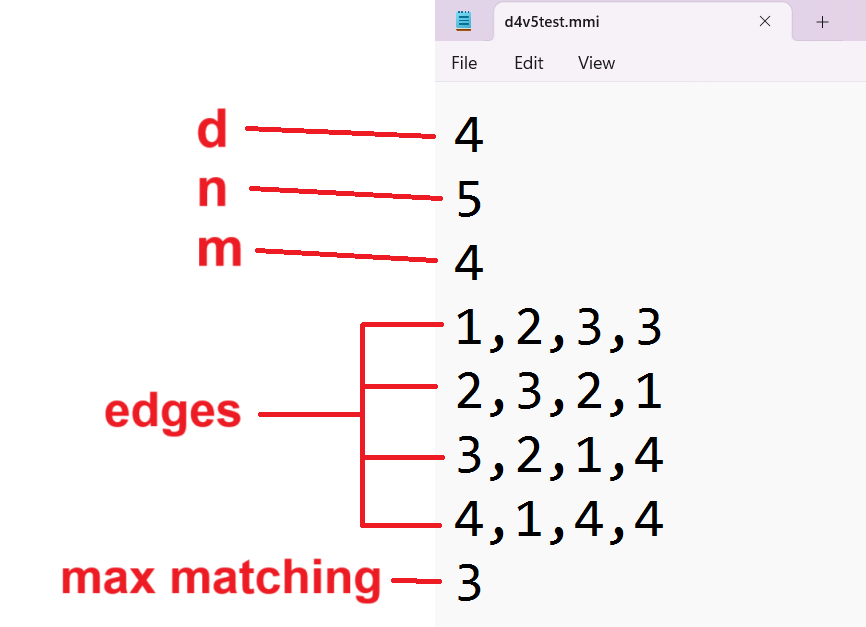
\includegraphics[width=\textwidth]{images/exampleMMI.png}
        \caption{An example of an .mmi instance. Each line is labeled with the information
        it contains. Note that the file represents some information that is not stated by 
        just the edges, such as the fact there is a 5th row of vertices that no edge visits.}
        \label{fig:exampleMMi}
    \end{minipage}
    \hfill
\end{figure}

\begin{figure}[t!]
    \centering
    \begin{minipage}{0.45\textwidth}
        \centering
        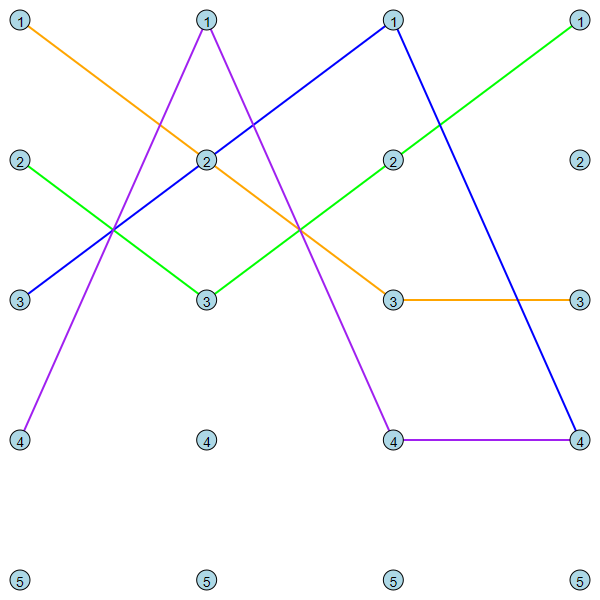
\includegraphics[width=\textwidth]{images/d4v5test.png}
        \caption{An example of a graph represented in a .mmi file.}
        \label{fig:d4v5}
    \end{minipage}
    \hfill
\end{figure}

A .mmb files contains a series of paths to .mmi files. Each line contains a path to 
a .mmi file or a series of .mmi files. Note that .mmb supports wildcards, which are
represented as a *. This means that one line in .mmb file can lead to many 
different .mmi files. This is useful for including all .mmi files in a folder,
which is often the case for test suites. 

\section{Solvers} \label{SolverSummary}
There are many solvers in our implementation. Each solver takes in a graph instance
as described in Section \ref{BenchmarkingSummary} and returns a list of edges representing
a maximum matching on the graph instance. We implement many different algorithms and 
programming styles to find efficient ways of finding the maximum matching. 
The following is a list of the
different types of solver implemented over the course of the project:
\begin{itemize}
    \item Edmonds-Karp 
    \item Hopcroft-Karp
    \item Brute Force
    \item A*
    \item Depth First Search
    \item Integer Programming
    \item Parallel Programming
    \item Approximate solvers
\end{itemize}
For more information on the implementation of solvers and an example of an implemented solver,
see Section \ref{ekImplement}.

\section{Test Generators}
Each solver needs to be tested against a large variety of .mmi files. This is
done to determine not only the accuracy, but also the running time. There are 
currently two test generators in our implementation: a Brute Force verified 
generator, and a strategic $d > 2$ generator. For more details, see Section \ref{StrategicRandomTest}. Each generator provides
a way to randomly generate graphs with known maximum matching sizes. We compare 
the cardinality of the set of edges returned by each solver to the known cardinality of
the maximum matching to
determine accuracy. Being able to produce large groups of graphs also allows for 
diverse test suites to be generated. We then generate courses
for determining running time using the benchmarking programs, as seen in 
Section \ref{BenchmarkingSummary}. 

\section{Visualizer}
A visualizer allows for .mmi files to be more easily understandable to a human 
audience. The visualizer utilizes the graph framework provided for by igraph and 
pycairo. Each visualization is a .png that represents each dimension as a column with each vertex of the same value on the same row. Hyperedges are represented by
different color lines for ease of recognition.

The visualizer visualizes graphs by parsing a .mmi file and then converting the information
into a pycario graph object. Note that pycario does not support d-partite graphs or hyperedges,
so the visualizer adds vertices and edges to the graph object to emulate them.

\begin{figure}[t!]
    \centering
    \begin{minipage}{0.45\textwidth}
        \centering
        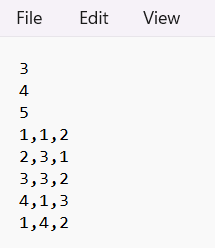
\includegraphics[width=\textwidth]{images/exampleviz.png}
        \caption{An example .mmi file to visualize.}
        \label{fig:vizbase}
    \end{minipage}
    \hfill
\end{figure}

\begin{figure}[t!]
    \centering
    \begin{minipage}{0.45\textwidth}
        \centering
        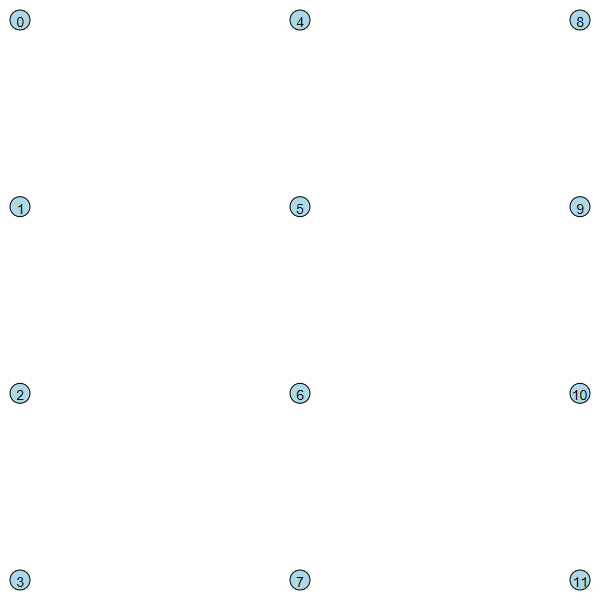
\includegraphics[width=\textwidth]{images/viz0.png}
        \caption{An example of how nodes are actually represented in the pycairo graph object in the visualizer. Note how nodes are labeled starting from 0 and increasing by 1. Uses the information given in Figure \ref{fig:vizbase}}
        \label{fig:viz0}
    \end{minipage}
    \hfill
\end{figure}

First, the visualizer adds $d * n$ edges to the graph object. Pycario automatically adds 
labels to the vertices in order of their addition starting at 0. This is shown in Figure
\ref{fig:viz0}. We add custom labels to each vertex using the formula 
$new label$ $=(label \% n) + 1$. This can be seen in Figure \ref{fig:viz1}.

\begin{figure}[t!]
    \centering
    \begin{minipage}{0.45\textwidth}
        \centering
        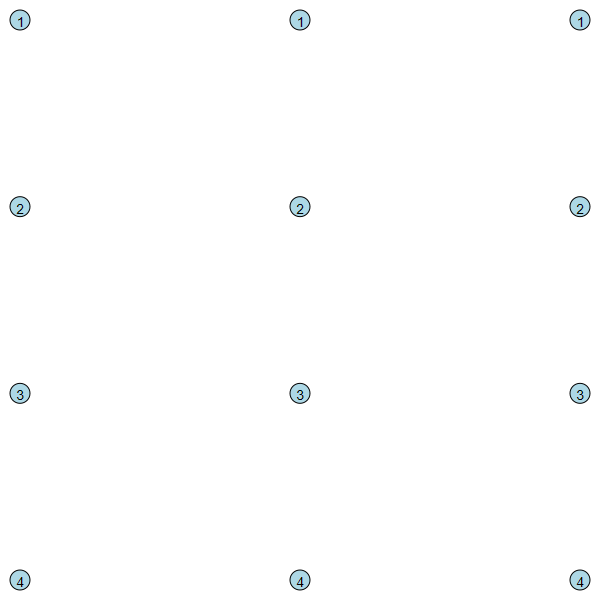
\includegraphics[width=\textwidth]{images/viz1.png}
        \caption{An example of how vertices are labeled in the visualizer. Continues from Figure \ref{fig:viz0}}
        \label{fig:viz1}
    \end{minipage}
    \hfill
\end{figure}

Edges are added in a similar manner. We add a hyperedge $e$ one edge at a time. We do this by 
adding edges using the formula $(((e[i] - 1) + n * i), ((e[i+1] - 1) + n * (i + 1)))$. We 
subtract 1 from the value at each index as pycario stores labels starting at 0, but we store
vertices starting from 1 in the .mmi file. We then add the $n * i$ to each vertex to 
place it in the correct dimension. This is seen in Figure \ref{fig:viz2}

\begin{figure}[t!]
    \centering
    \begin{minipage}{0.45\textwidth}
        \centering
        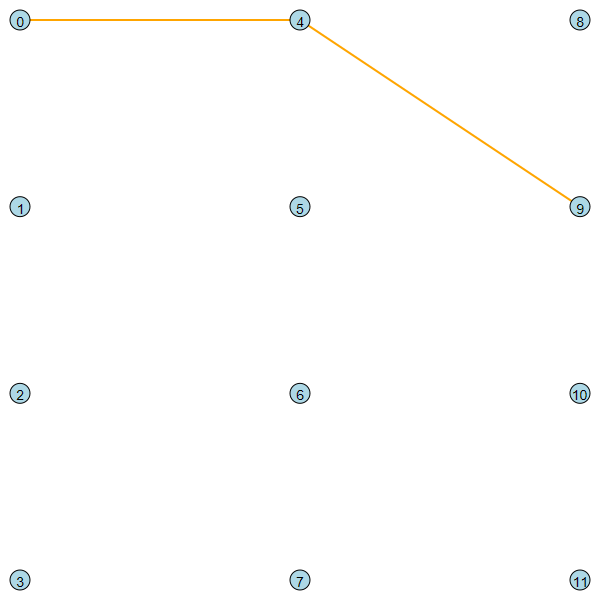
\includegraphics[width=\textwidth]{images/viz2.png}
        \caption{An example of how a single hyperedge is added to the visual. In this case, we are adding the hyper edge $(1, 1, 2)$. Using the formula, we first add the edge $(((e[0] - 1) + 4 * 0), ((e[0+1] - 1) + 4 * (0 + 1)))$. This gives us $((0 + 0), (0 + 4))$ or $(0,4)$. We then add the next edge in the hyperedge $(((e[1] - 1) + 4 * 1), ((e[1+1] - 1) + 4 * (1 + 1)))$ or $(4), (8)$. We then color the edges accordingly to represent the hyperedge.}
        \label{fig:viz2}
    \end{minipage}
    \hfill
\end{figure}

For ease of visual clarity, we also keep track of how many edges are represented in the 
hyperedge so that they can be colored accordingly. We repeat this for each hyperedge until 
there are no more hyperedges to draw as seen in Figure \ref{fig:viz3}.

\begin{figure}[t!]
    \centering
    \begin{minipage}{0.45\textwidth}
        \centering
        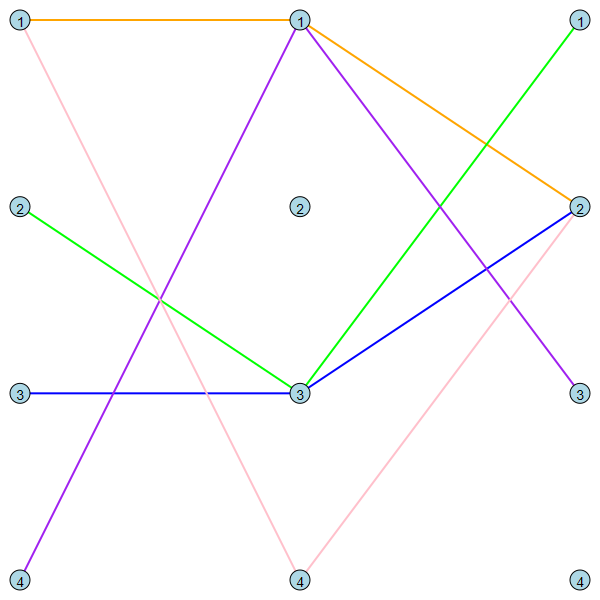
\includegraphics[width=\textwidth]{images/viz3.png}
        \caption{A completed visualization of Figure \ref{fig:vizbase}}
        \label{fig:viz3}
    \end{minipage}
    \hfill
\end{figure}
